\chapter{Ergebnisse}
\label{cha:umsetzung}
\section{Umsetzung des Softwaredesigns auf den Mikrocontrollern}
\label{sec:Node-MCU}

\subsection*{Softwarearchitektur und Designtools}

\subsection*{Startup der MCU-Controller}



\autoref{lst:assembling_mqtt_receive}

\section{Visualisierung der Prozessdaten in Node-RED}
\label{sec:Node-Red}

\begin{figure}[H]
	\centering
	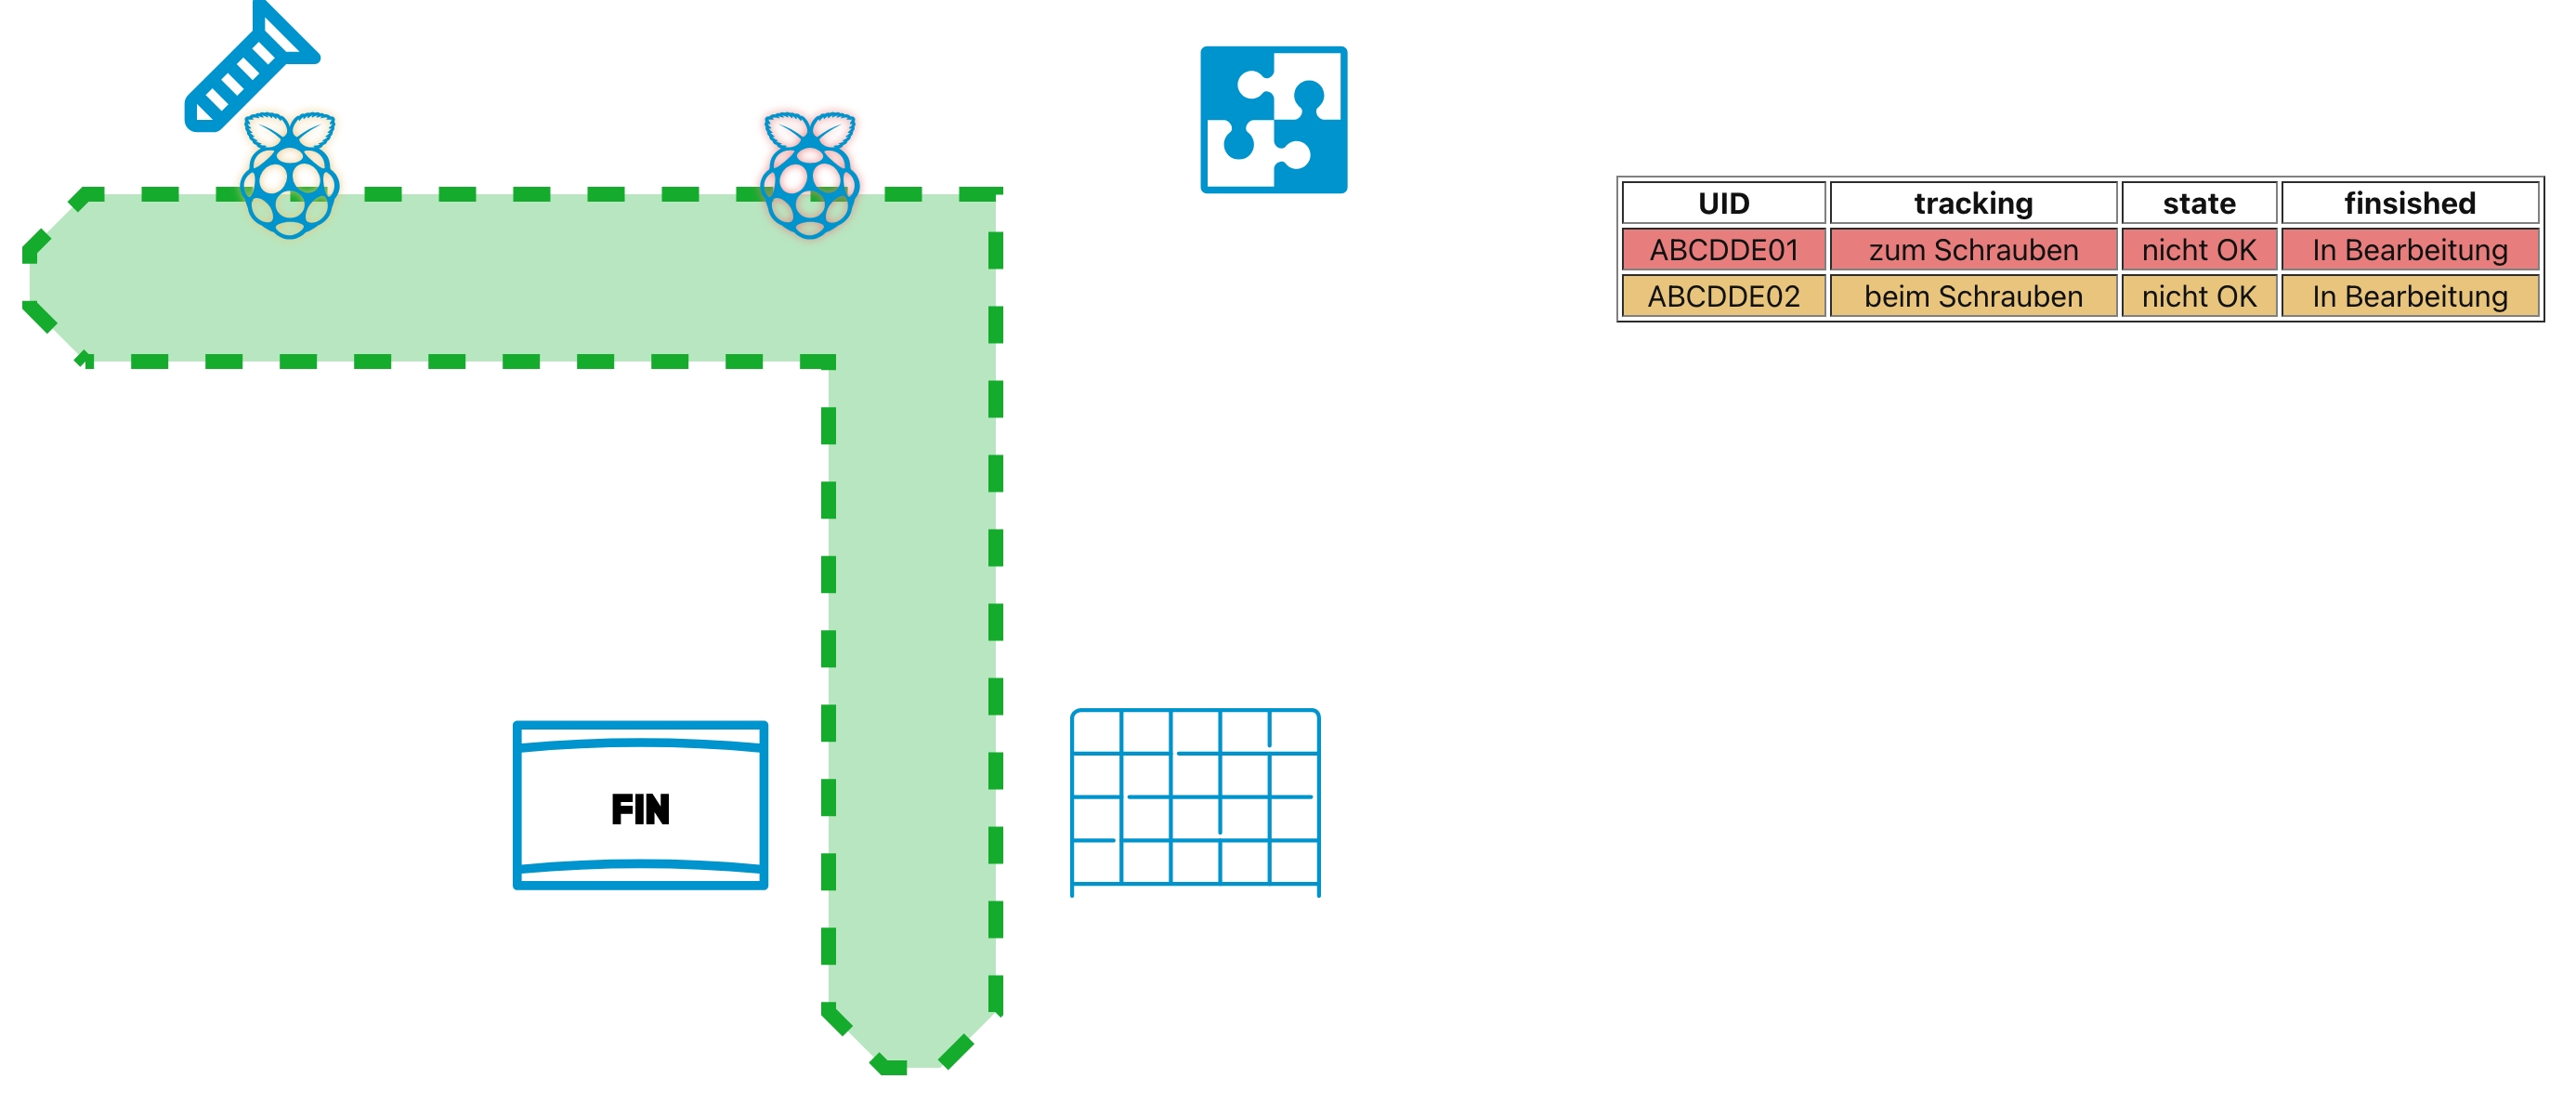
\includegraphics[width=0.8\textwidth]{images/node-red-band.jpeg}
	\caption{Node-RED-Dashboard des NFC-Tracking-Systems}
	\label{fig:dashboard}
\end{figure}

Zur Visualisierung der Produktpositionen und -zustände innerhalb des Bandumlaufsystems wurde ein interaktives Dashboard mit Node-RED implementiert (siehe \autoref{fig:dashboard}). Dieses Dashboard stellt die vier Stationen geometrisch entsprechend ihrer Anordnung in der Lernfabrik dar. Produkte werden symbolisch als Raspberry-Pi-Icons dargestellt und entlang des virtuellen Förderbands basierend auf ihrem erfassten Tracking-Zustand positioniert.

Die aktuelle Systemübersicht umfasst zwei Hauptkomponenten:
\begin{itemize}
	\item \textbf{Visuelle Darstellung des Förderbands:} Produkte bewegen sich entsprechend ihres Zustands zwischen den Stationen.
	\item \textbf{Tabelle mit Produktinformationen:} Für jedes Produkt wird eine eindeutige UID sowie der aktuelle Tracking-Zustand, der letzte Bearbeitungsstatus und ein Fertigstellungsindikator angezeigt. Die Zeilen sind farblich codiert, um die visuelle Unterscheidbarkeit der Produkte zu erhöhen.
\end{itemize}

\begin{figure}[H]
	\centering
	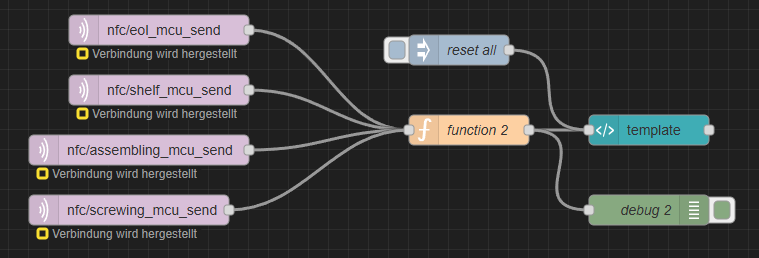
\includegraphics[width=0.8\textwidth]{images/node-red-flow-receive.png}
	\caption{Node-RED-Flow zum Empfang von Nachrichten}
	\label{fig:receive_nodes}
\end{figure}

Node-RED ermöglicht eine visuelle und modulare Abbildung der Prozesslogik. Die Empfangslogik ist in \autoref{fig:receive_nodes} dargestellt. Dabei werden vier verschiedene MQTT-Topics abonniert, über die jeweils eine der vier Stationen Nachrichten an das zentrale System sendet. Die empfangenen JSON-Daten werden über \texttt{MQTT-IN}-Nodes verarbeitet und anschließend von \texttt{Function}-Nodes analysiert. Die Logik in diesen Funktionsbausteinen umfasst:
\begin{itemize}
	\item Zuordnung der Nachricht zur entsprechenden Station
	\item Berechnung der exakten Position auf dem Dashboard
	\item Generierung einer individuellen Tabellenfarbe pro UID
\end{itemize}

Zusätzlich enthält der Flow einen Reset-Node zum Zurücksetzen des Dashboards sowie einen Debug-Node zur Laufzeitanalyse.

\begin{figure}[H]
	\centering
	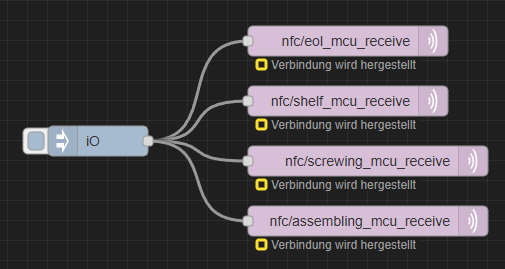
\includegraphics[width=0.8\textwidth]{images/node-red-flow-send.png}
	\caption{Node-RED-Flow zum Senden von Nachrichten an Stationen}
	\label{fig:send_nodes}
\end{figure}

Für Testzwecke wurde ein dedizierter Sende-Flow implementiert (\autoref{fig:send_nodes}). Dieser ermöglicht das manuelle Senden von Steuerinformationen an die Mikrocontroller an den Stationen über vier weitere MQTT-Topics. Diese haben dieselbe Namenskonvention wie die Empfangs-Topics, enthalten jedoch den Suffix \texttt{\_receive} anstelle von \texttt{\_send}. So kann eine einfache manuelle Steuerung einzelner Produktzustände direkt aus dem Dashboard heraus erfolgen.

\begin{table}[H]
	\centering
	\caption{MQTT-Topics}
	\label{tab:mqtt_topics}
	\begin{tabular}{|c|l|}
		\hline
		\textbf{Topic} & \textbf{Beschreibung} \\ \hline
		$rfid/eol\_mcu\_send$ & Datenübertragung von der EOL-Station zum Dashboard \\ 
		$rfid/shelf\_mcu\_send$ & Datenübertragung von der Lagerstation zum Dashboard \\ 
		$rfid/assembling\_mcu\_send$ & Datenübertragung von der Montage-Station zum Dashboard \\ 
		$rfid/screwing\_mcu\_send$ & Datenübertragung von der Schraubstation zum Dashboard \\ \hline
		$rfid/eol\_mcu\_receive$ & Steuerbefehl an die EOL-Station \\ 
		$rfid/shelf\_mcu\_receive$ & Steuerbefehl an die Lagerstation \\ 
		$rfid/assembling\_mcu\_receive$ & Steuerbefehl an die Montage-Station \\ 
		$rfid/screwing\_mcu\_receive$ & Steuerbefehl an die Schraubstation \\ \hline
	\end{tabular}
\end{table}


